\section{Further question: the two regimes scale on different bottlenecks}
\label{sec:scaling}

The framework invites a scaling question it does not answer, and unpacking the bundle
changes what the question is. The two corners do not grow along the same variable, so they
cannot degrade for the same reason.

A public network grows in $N$, the number of addressable counterparts, and $N$ is not
chosen by anyone. Coverage rises with it; so do search cost, verification cost and
exposure to counterparts nobody vetted. Its binding constraint is whether ranking can still
surface the right counterpart out of $N$.

A private network cannot grow in $N$: a roster is bounded by construction. It grows in
$d$, the number of brokered hops a request may travel, because that is the only way trusted
coverage increases. Its costs are not retrieval costs---they are the cost of asking a
broker to spend its own standing, and the decay of whatever recourse survives a chain of
introductions. Its binding constraint is path length and trust transitivity.

\begin{quote}
\textbf{Public networks scale through ranking; private networks scale through
relationships.} The open question the framework poses is not which is better at scale but
which degrades faster, under what task distribution, and whether a hybrid inherits the
better bottleneck from each.
\end{quote}

We can speak to the first of the two and not the second.

Within the range we can run, directory size does nothing. Growing the directory from 50
to 800 cards---16$\times$, with the roster held at twenty---leaves the open arm's score
flat ($0.800 \to 0.826$, CI spans zero) while search precision falls by roughly half and
tokens double. The arm pays for the extra difficulty rather than failing at it. We report
this null with a caveat earned the hard way: our first reading of this sweep was a
scaling result, and it was an outage (Appendix~\ref{app:retracted}).


\begin{figure}[t]
\centering
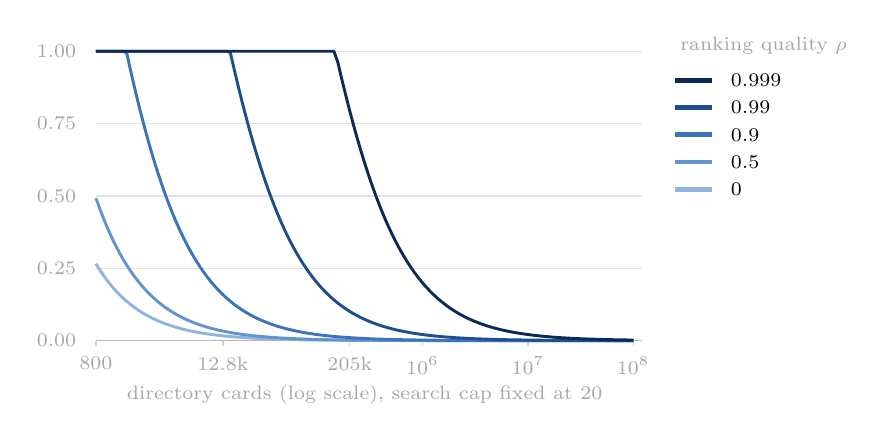
\begin{tikzpicture}[x=1.05cm,y=1.05cm,font=\small]
\draw[gray!22] (0,0.000) -- (6.60,0.000);
\node[gray!70,font=\scriptsize,anchor=east] at (-0.12,0.000) {0.00};
\draw[gray!22] (0,0.875) -- (6.60,0.875);
\node[gray!70,font=\scriptsize,anchor=east] at (-0.12,0.875) {0.25};
\draw[gray!22] (0,1.750) -- (6.60,1.750);
\node[gray!70,font=\scriptsize,anchor=east] at (-0.12,1.750) {0.50};
\draw[gray!22] (0,2.625) -- (6.60,2.625);
\node[gray!70,font=\scriptsize,anchor=east] at (-0.12,2.625) {0.75};
\draw[gray!22] (0,3.500) -- (6.60,3.500);
\node[gray!70,font=\scriptsize,anchor=east] at (-0.12,3.500) {1.00};
\draw[gray!55] (0,0) -- (6.60,0);
\draw[gray!35] (0.000,0) -- (0.000,-0.07);
\node[gray!70,font=\scriptsize,anchor=north] at (0.000,-0.08) {800};
\draw[gray!35] (1.536,0) -- (1.536,-0.07);
\node[gray!70,font=\scriptsize,anchor=north] at (1.536,-0.08) {12.8k};
\draw[gray!35] (3.071,0) -- (3.071,-0.07);
\node[gray!70,font=\scriptsize,anchor=north] at (3.071,-0.08) {205k};
\draw[gray!35] (3.949,0) -- (3.949,-0.07);
\node[gray!70,font=\scriptsize,anchor=north] at (3.949,-0.08) {$10^6$};
\draw[gray!35] (5.225,0) -- (5.225,-0.07);
\node[gray!70,font=\scriptsize,anchor=north] at (5.225,-0.08) {$10^7$};
\draw[gray!35] (6.500,0) -- (6.500,-0.07);
\node[gray!70,font=\scriptsize,anchor=north] at (6.500,-0.08) {$10^8$};
\definecolor{rc0}{HTML}{8FB4DE}
\definecolor{rc0p5}{HTML}{6394CE}
\definecolor{rc0p9}{HTML}{3B74BC}
\definecolor{rc0p99}{HTML}{1E4E8C}
\definecolor{rc0p999}{HTML}{0C2B54}
\draw[rc0,line width=1.05pt,line join=round] (0.0000,0.9309) -- (0.0464,0.8560) -- (0.0929,0.7872) -- (0.1393,0.7239) -- (0.1857,0.6657) -- (0.2321,0.6121) -- (0.2786,0.5629) -- (0.3250,0.5176) -- (0.3714,0.4760) -- (0.4179,0.4377) -- (0.4643,0.4025) -- (0.5107,0.3702) -- (0.5571,0.3404) -- (0.6036,0.3130) -- (0.6500,0.2879) -- (0.6964,0.2647) -- (0.7429,0.2434) -- (0.7893,0.2239) -- (0.8357,0.2059) -- (0.8821,0.1893) -- (0.9286,0.1741) -- (0.9750,0.1601) -- (1.0214,0.1472) -- (1.0679,0.1354) -- (1.1143,0.1245) -- (1.1607,0.1145) -- (1.2071,0.1053) -- (1.2536,0.0968) -- (1.3000,0.0890) -- (1.3464,0.0819) -- (1.3929,0.0753) -- (1.4393,0.0692) -- (1.4857,0.0637) -- (1.5321,0.0585) -- (1.5786,0.0538) -- (1.6250,0.0495) -- (1.6714,0.0455) -- (1.7179,0.0419) -- (1.7643,0.0385) -- (1.8107,0.0354) -- (1.8571,0.0326) -- (1.9036,0.0299) -- (1.9500,0.0275) -- (1.9964,0.0253) -- (2.0429,0.0233) -- (2.0893,0.0214) -- (2.1357,0.0197) -- (2.1821,0.0181) -- (2.2286,0.0166) -- (2.2750,0.0153) -- (2.3214,0.0141) -- (2.3679,0.0129) -- (2.4143,0.0119) -- (2.4607,0.0109) -- (2.5071,0.0101) -- (2.5536,0.0093) -- (2.6000,0.0085) -- (2.6464,0.0078) -- (2.6929,0.0072) -- (2.7393,0.0066) -- (2.7857,0.0061) -- (2.8321,0.0056) -- (2.8786,0.0051) -- (2.9250,0.0047) -- (2.9714,0.0044) -- (3.0179,0.0040) -- (3.0643,0.0037) -- (3.1107,0.0034) -- (3.1571,0.0031) -- (3.2036,0.0029) -- (3.2500,0.0026) -- (3.2964,0.0024) -- (3.3429,0.0022) -- (3.3893,0.0020) -- (3.4357,0.0019) -- (3.4821,0.0017) -- (3.5286,0.0016) -- (3.5750,0.0015) -- (3.6214,0.0013) -- (3.6679,0.0012) -- (3.7143,0.0011) -- (3.7607,0.0010) -- (3.8071,0.0010) -- (3.8536,0.0009) -- (3.9000,0.0008) -- (3.9464,0.0007) -- (3.9929,0.0007) -- (4.0393,0.0006) -- (4.0857,0.0006) -- (4.1321,0.0005) -- (4.1786,0.0005) -- (4.2250,0.0005) -- (4.2714,0.0004) -- (4.3179,0.0004) -- (4.3643,0.0004) -- (4.4107,0.0003) -- (4.4571,0.0003) -- (4.5036,0.0003) -- (4.5500,0.0003) -- (4.5964,0.0002) -- (4.6429,0.0002) -- (4.6893,0.0002) -- (4.7357,0.0002) -- (4.7821,0.0002) -- (4.8286,0.0002) -- (4.8750,0.0001) -- (4.9214,0.0001) -- (4.9679,0.0001) -- (5.0143,0.0001) -- (5.0607,0.0001) -- (5.1071,0.0001) -- (5.1536,0.0001) -- (5.2000,0.0001) -- (5.2464,0.0001) -- (5.2929,0.0001) -- (5.3393,0.0001) -- (5.3857,0.0001) -- (5.4321,0.0001) -- (5.4786,0.0000) -- (5.5250,0.0000) -- (5.5714,0.0000) -- (5.6179,0.0000) -- (5.6643,0.0000) -- (5.7107,0.0000) -- (5.7571,0.0000) -- (5.8036,0.0000) -- (5.8500,0.0000) -- (5.8964,0.0000) -- (5.9429,0.0000) -- (5.9893,0.0000) -- (6.0357,0.0000) -- (6.0821,0.0000) -- (6.1286,0.0000) -- (6.1750,0.0000) -- (6.2214,0.0000) -- (6.2679,0.0000) -- (6.3143,0.0000) -- (6.3607,0.0000) -- (6.4071,0.0000) -- (6.4536,0.0000) -- (6.5000,0.0000);
\draw[rc0p5,line width=1.05pt,line join=round] (0.0000,1.7241) -- (0.0464,1.5950) -- (0.0929,1.4748) -- (0.1393,1.3632) -- (0.1857,1.2595) -- (0.2321,1.1632) -- (0.2786,1.0740) -- (0.3250,0.9913) -- (0.3714,0.9147) -- (0.4179,0.8438) -- (0.4643,0.7782) -- (0.5107,0.7176) -- (0.5571,0.6615) -- (0.6036,0.6097) -- (0.6500,0.5619) -- (0.6964,0.5177) -- (0.7429,0.4769) -- (0.7893,0.4393) -- (0.8357,0.4046) -- (0.8821,0.3726) -- (0.9286,0.3430) -- (0.9750,0.3158) -- (1.0214,0.2908) -- (1.0679,0.2676) -- (1.1143,0.2463) -- (1.1607,0.2267) -- (1.2071,0.2087) -- (1.2536,0.1920) -- (1.3000,0.1767) -- (1.3464,0.1626) -- (1.3929,0.1496) -- (1.4393,0.1376) -- (1.4857,0.1266) -- (1.5321,0.1165) -- (1.5786,0.1072) -- (1.6250,0.0986) -- (1.6714,0.0907) -- (1.7179,0.0834) -- (1.7643,0.0767) -- (1.8107,0.0706) -- (1.8571,0.0649) -- (1.9036,0.0597) -- (1.9500,0.0549) -- (1.9964,0.0505) -- (2.0429,0.0465) -- (2.0893,0.0427) -- (2.1357,0.0393) -- (2.1821,0.0362) -- (2.2286,0.0332) -- (2.2750,0.0306) -- (2.3214,0.0281) -- (2.3679,0.0259) -- (2.4143,0.0238) -- (2.4607,0.0219) -- (2.5071,0.0201) -- (2.5536,0.0185) -- (2.6000,0.0170) -- (2.6464,0.0156) -- (2.6929,0.0144) -- (2.7393,0.0132) -- (2.7857,0.0122) -- (2.8321,0.0112) -- (2.8786,0.0103) -- (2.9250,0.0095) -- (2.9714,0.0087) -- (3.0179,0.0080) -- (3.0643,0.0074) -- (3.1107,0.0068) -- (3.1571,0.0062) -- (3.2036,0.0057) -- (3.2500,0.0053) -- (3.2964,0.0048) -- (3.3429,0.0045) -- (3.3893,0.0041) -- (3.4357,0.0038) -- (3.4821,0.0035) -- (3.5286,0.0032) -- (3.5750,0.0029) -- (3.6214,0.0027) -- (3.6679,0.0025) -- (3.7143,0.0023) -- (3.7607,0.0021) -- (3.8071,0.0019) -- (3.8536,0.0018) -- (3.9000,0.0016) -- (3.9464,0.0015) -- (3.9929,0.0014) -- (4.0393,0.0013) -- (4.0857,0.0012) -- (4.1321,0.0011) -- (4.1786,0.0010) -- (4.2250,0.0009) -- (4.2714,0.0008) -- (4.3179,0.0008) -- (4.3643,0.0007) -- (4.4107,0.0006) -- (4.4571,0.0006) -- (4.5036,0.0005) -- (4.5500,0.0005) -- (4.5964,0.0005) -- (4.6429,0.0004) -- (4.6893,0.0004) -- (4.7357,0.0004) -- (4.7821,0.0003) -- (4.8286,0.0003) -- (4.8750,0.0003) -- (4.9214,0.0003) -- (4.9679,0.0002) -- (5.0143,0.0002) -- (5.0607,0.0002) -- (5.1071,0.0002) -- (5.1536,0.0002) -- (5.2000,0.0002) -- (5.2464,0.0001) -- (5.2929,0.0001) -- (5.3393,0.0001) -- (5.3857,0.0001) -- (5.4321,0.0001) -- (5.4786,0.0001) -- (5.5250,0.0001) -- (5.5714,0.0001) -- (5.6179,0.0001) -- (5.6643,0.0001) -- (5.7107,0.0001) -- (5.7571,0.0001) -- (5.8036,0.0001) -- (5.8500,0.0000) -- (5.8964,0.0000) -- (5.9429,0.0000) -- (5.9893,0.0000) -- (6.0357,0.0000) -- (6.0821,0.0000) -- (6.1286,0.0000) -- (6.1750,0.0000) -- (6.2214,0.0000) -- (6.2679,0.0000) -- (6.3143,0.0000) -- (6.3607,0.0000) -- (6.4071,0.0000) -- (6.4536,0.0000) -- (6.5000,0.0000);
\draw[rc0p9,line width=1.05pt,line join=round] (0.0000,3.5000) -- (0.0464,3.5000) -- (0.0929,3.5000) -- (0.1393,3.5000) -- (0.1857,3.5000) -- (0.2321,3.5000) -- (0.2786,3.5000) -- (0.3250,3.5000) -- (0.3714,3.4817) -- (0.4179,3.2724) -- (0.4643,3.0716) -- (0.5107,2.8795) -- (0.5571,2.6961) -- (0.6036,2.5215) -- (0.6500,2.3556) -- (0.6964,2.1983) -- (0.7429,2.0494) -- (0.7893,1.9089) -- (0.8357,1.7765) -- (0.8821,1.6518) -- (0.9286,1.5347) -- (0.9750,1.4249) -- (1.0214,1.3220) -- (1.0679,1.2257) -- (1.1143,1.1358) -- (1.1607,1.0519) -- (1.2071,0.9736) -- (1.2536,0.9008) -- (1.3000,0.8330) -- (1.3464,0.7700) -- (1.3929,0.7115) -- (1.4393,0.6572) -- (1.4857,0.6068) -- (1.5321,0.5601) -- (1.5786,0.5169) -- (1.6250,0.4768) -- (1.6714,0.4398) -- (1.7179,0.4055) -- (1.7643,0.3739) -- (1.8107,0.3446) -- (1.8571,0.3176) -- (1.9036,0.2926) -- (1.9500,0.2696) -- (1.9964,0.2483) -- (2.0429,0.2287) -- (2.0893,0.2106) -- (2.1357,0.1939) -- (2.1821,0.1785) -- (2.2286,0.1644) -- (2.2750,0.1513) -- (2.3214,0.1393) -- (2.3679,0.1282) -- (2.4143,0.1180) -- (2.4607,0.1086) -- (2.5071,0.0999) -- (2.5536,0.0919) -- (2.6000,0.0846) -- (2.6464,0.0778) -- (2.6929,0.0716) -- (2.7393,0.0659) -- (2.7857,0.0606) -- (2.8321,0.0557) -- (2.8786,0.0513) -- (2.9250,0.0472) -- (2.9714,0.0434) -- (3.0179,0.0399) -- (3.0643,0.0367) -- (3.1107,0.0338) -- (3.1571,0.0311) -- (3.2036,0.0286) -- (3.2500,0.0263) -- (3.2964,0.0242) -- (3.3429,0.0222) -- (3.3893,0.0204) -- (3.4357,0.0188) -- (3.4821,0.0173) -- (3.5286,0.0159) -- (3.5750,0.0146) -- (3.6214,0.0135) -- (3.6679,0.0124) -- (3.7143,0.0114) -- (3.7607,0.0105) -- (3.8071,0.0096) -- (3.8536,0.0088) -- (3.9000,0.0081) -- (3.9464,0.0075) -- (3.9929,0.0069) -- (4.0393,0.0063) -- (4.0857,0.0058) -- (4.1321,0.0054) -- (4.1786,0.0049) -- (4.2250,0.0045) -- (4.2714,0.0042) -- (4.3179,0.0038) -- (4.3643,0.0035) -- (4.4107,0.0032) -- (4.4571,0.0030) -- (4.5036,0.0027) -- (4.5500,0.0025) -- (4.5964,0.0023) -- (4.6429,0.0021) -- (4.6893,0.0020) -- (4.7357,0.0018) -- (4.7821,0.0017) -- (4.8286,0.0015) -- (4.8750,0.0014) -- (4.9214,0.0013) -- (4.9679,0.0012) -- (5.0143,0.0011) -- (5.0607,0.0010) -- (5.1071,0.0009) -- (5.1536,0.0008) -- (5.2000,0.0008) -- (5.2464,0.0007) -- (5.2929,0.0007) -- (5.3393,0.0006) -- (5.3857,0.0006) -- (5.4321,0.0005) -- (5.4786,0.0005) -- (5.5250,0.0004) -- (5.5714,0.0004) -- (5.6179,0.0004) -- (5.6643,0.0003) -- (5.7107,0.0003) -- (5.7571,0.0003) -- (5.8036,0.0003) -- (5.8500,0.0002) -- (5.8964,0.0002) -- (5.9429,0.0002) -- (5.9893,0.0002) -- (6.0357,0.0002) -- (6.0821,0.0002) -- (6.1286,0.0001) -- (6.1750,0.0001) -- (6.2214,0.0001) -- (6.2679,0.0001) -- (6.3143,0.0001) -- (6.3607,0.0001) -- (6.4071,0.0001) -- (6.4536,0.0001) -- (6.5000,0.0001);
\draw[rc0p99,line width=1.05pt,line join=round] (0.0000,3.5000) -- (0.0464,3.5000) -- (0.0929,3.5000) -- (0.1393,3.5000) -- (0.1857,3.5000) -- (0.2321,3.5000) -- (0.2786,3.5000) -- (0.3250,3.5000) -- (0.3714,3.5000) -- (0.4179,3.5000) -- (0.4643,3.5000) -- (0.5107,3.5000) -- (0.5571,3.5000) -- (0.6036,3.5000) -- (0.6500,3.5000) -- (0.6964,3.5000) -- (0.7429,3.5000) -- (0.7893,3.5000) -- (0.8357,3.5000) -- (0.8821,3.5000) -- (0.9286,3.5000) -- (0.9750,3.5000) -- (1.0214,3.5000) -- (1.0679,3.5000) -- (1.1143,3.5000) -- (1.1607,3.5000) -- (1.2071,3.5000) -- (1.2536,3.5000) -- (1.3000,3.5000) -- (1.3464,3.5000) -- (1.3929,3.5000) -- (1.4393,3.5000) -- (1.4857,3.5000) -- (1.5321,3.5000) -- (1.5786,3.5000) -- (1.6250,3.4861) -- (1.6714,3.2839) -- (1.7179,3.0890) -- (1.7643,2.9018) -- (1.8107,2.7224) -- (1.8571,2.5508) -- (1.9036,2.3873) -- (1.9500,2.2317) -- (1.9964,2.0839) -- (2.0429,1.9440) -- (2.0893,1.8117) -- (2.1357,1.6869) -- (2.1821,1.5693) -- (2.2286,1.4587) -- (2.2750,1.3549) -- (2.3214,1.2576) -- (2.3679,1.1665) -- (2.4143,1.0813) -- (2.4607,1.0017) -- (2.5071,0.9275) -- (2.5536,0.8584) -- (2.6000,0.7940) -- (2.6464,0.7341) -- (2.6929,0.6785) -- (2.7393,0.6268) -- (2.7857,0.5789) -- (2.8321,0.5345) -- (2.8786,0.4933) -- (2.9250,0.4552) -- (2.9714,0.4199) -- (3.0179,0.3872) -- (3.0643,0.3570) -- (3.1107,0.3291) -- (3.1571,0.3033) -- (3.2036,0.2795) -- (3.2500,0.2575) -- (3.2964,0.2372) -- (3.3429,0.2185) -- (3.3893,0.2012) -- (3.4357,0.1853) -- (3.4821,0.1706) -- (3.5286,0.1571) -- (3.5750,0.1446) -- (3.6214,0.1331) -- (3.6679,0.1225) -- (3.7143,0.1128) -- (3.7607,0.1038) -- (3.8071,0.0955) -- (3.8536,0.0879) -- (3.9000,0.0809) -- (3.9464,0.0744) -- (3.9929,0.0685) -- (4.0393,0.0630) -- (4.0857,0.0579) -- (4.1321,0.0533) -- (4.1786,0.0490) -- (4.2250,0.0451) -- (4.2714,0.0415) -- (4.3179,0.0382) -- (4.3643,0.0351) -- (4.4107,0.0323) -- (4.4571,0.0297) -- (4.5036,0.0273) -- (4.5500,0.0251) -- (4.5964,0.0231) -- (4.6429,0.0213) -- (4.6893,0.0195) -- (4.7357,0.0180) -- (4.7821,0.0165) -- (4.8286,0.0152) -- (4.8750,0.0140) -- (4.9214,0.0129) -- (4.9679,0.0118) -- (5.0143,0.0109) -- (5.0607,0.0100) -- (5.1071,0.0092) -- (5.1536,0.0085) -- (5.2000,0.0078) -- (5.2464,0.0072) -- (5.2929,0.0066) -- (5.3393,0.0061) -- (5.3857,0.0056) -- (5.4321,0.0051) -- (5.4786,0.0047) -- (5.5250,0.0043) -- (5.5714,0.0040) -- (5.6179,0.0037) -- (5.6643,0.0034) -- (5.7107,0.0031) -- (5.7571,0.0028) -- (5.8036,0.0026) -- (5.8500,0.0024) -- (5.8964,0.0022) -- (5.9429,0.0020) -- (5.9893,0.0019) -- (6.0357,0.0017) -- (6.0821,0.0016) -- (6.1286,0.0015) -- (6.1750,0.0013) -- (6.2214,0.0012) -- (6.2679,0.0011) -- (6.3143,0.0010) -- (6.3607,0.0010) -- (6.4071,0.0009) -- (6.4536,0.0008) -- (6.5000,0.0007);
\draw[rc0p999,line width=1.05pt,line join=round] (0.0000,3.5000) -- (0.0464,3.5000) -- (0.0929,3.5000) -- (0.1393,3.5000) -- (0.1857,3.5000) -- (0.2321,3.5000) -- (0.2786,3.5000) -- (0.3250,3.5000) -- (0.3714,3.5000) -- (0.4179,3.5000) -- (0.4643,3.5000) -- (0.5107,3.5000) -- (0.5571,3.5000) -- (0.6036,3.5000) -- (0.6500,3.5000) -- (0.6964,3.5000) -- (0.7429,3.5000) -- (0.7893,3.5000) -- (0.8357,3.5000) -- (0.8821,3.5000) -- (0.9286,3.5000) -- (0.9750,3.5000) -- (1.0214,3.5000) -- (1.0679,3.5000) -- (1.1143,3.5000) -- (1.1607,3.5000) -- (1.2071,3.5000) -- (1.2536,3.5000) -- (1.3000,3.5000) -- (1.3464,3.5000) -- (1.3929,3.5000) -- (1.4393,3.5000) -- (1.4857,3.5000) -- (1.5321,3.5000) -- (1.5786,3.5000) -- (1.6250,3.5000) -- (1.6714,3.5000) -- (1.7179,3.5000) -- (1.7643,3.5000) -- (1.8107,3.5000) -- (1.8571,3.5000) -- (1.9036,3.5000) -- (1.9500,3.5000) -- (1.9964,3.5000) -- (2.0429,3.5000) -- (2.0893,3.5000) -- (2.1357,3.5000) -- (2.1821,3.5000) -- (2.2286,3.5000) -- (2.2750,3.5000) -- (2.3214,3.5000) -- (2.3679,3.5000) -- (2.4143,3.5000) -- (2.4607,3.5000) -- (2.5071,3.5000) -- (2.5536,3.5000) -- (2.6000,3.5000) -- (2.6464,3.5000) -- (2.6929,3.5000) -- (2.7393,3.5000) -- (2.7857,3.5000) -- (2.8321,3.5000) -- (2.8786,3.5000) -- (2.9250,3.3688) -- (2.9714,3.1714) -- (3.0179,2.9815) -- (3.0643,2.7992) -- (3.1107,2.6247) -- (3.1571,2.4581) -- (3.2036,2.2994) -- (3.2500,2.1485) -- (3.2964,2.0054) -- (3.3429,1.8699) -- (3.3893,1.7420) -- (3.4357,1.6214) -- (3.4821,1.5078) -- (3.5286,1.4011) -- (3.5750,1.3010) -- (3.6214,1.2072) -- (3.6679,1.1194) -- (3.7143,1.0374) -- (3.7607,0.9609) -- (3.8071,0.8895) -- (3.8536,0.8230) -- (3.9000,0.7611) -- (3.9464,0.7036) -- (3.9929,0.6502) -- (4.0393,0.6006) -- (4.0857,0.5546) -- (4.1321,0.5120) -- (4.1786,0.4725) -- (4.2250,0.4359) -- (4.2714,0.4020) -- (4.3179,0.3707) -- (4.3643,0.3418) -- (4.4107,0.3151) -- (4.4571,0.2904) -- (4.5036,0.2675) -- (4.5500,0.2465) -- (4.5964,0.2270) -- (4.6429,0.2091) -- (4.6893,0.1926) -- (4.7357,0.1773) -- (4.7821,0.1633) -- (4.8286,0.1503) -- (4.8750,0.1384) -- (4.9214,0.1274) -- (4.9679,0.1172) -- (5.0143,0.1079) -- (5.0607,0.0993) -- (5.1071,0.0914) -- (5.1536,0.0841) -- (5.2000,0.0774) -- (5.2464,0.0712) -- (5.2929,0.0655) -- (5.3393,0.0602) -- (5.3857,0.0554) -- (5.4321,0.0510) -- (5.4786,0.0469) -- (5.5250,0.0431) -- (5.5714,0.0397) -- (5.6179,0.0365) -- (5.6643,0.0336) -- (5.7107,0.0309) -- (5.7571,0.0284) -- (5.8036,0.0261) -- (5.8500,0.0240) -- (5.8964,0.0221) -- (5.9429,0.0203) -- (5.9893,0.0187) -- (6.0357,0.0172) -- (6.0821,0.0158) -- (6.1286,0.0145) -- (6.1750,0.0134) -- (6.2214,0.0123) -- (6.2679,0.0113) -- (6.3143,0.0104) -- (6.3607,0.0096) -- (6.4071,0.0088) -- (6.4536,0.0081) -- (6.5000,0.0074);
\node[gray!70,font=\scriptsize,anchor=west] at (6.95,3.570) {ranking quality $\rho$};
\draw[rc0p999,line width=1.7pt] (7.00,3.150) -- (7.45,3.150);
\node[font=\scriptsize,anchor=west] at (7.56,3.150) {$0.999$};
\draw[rc0p99,line width=1.7pt] (7.00,2.820) -- (7.45,2.820);
\node[font=\scriptsize,anchor=west] at (7.56,2.820) {$0.99$};
\draw[rc0p9,line width=1.7pt] (7.00,2.490) -- (7.45,2.490);
\node[font=\scriptsize,anchor=west] at (7.56,2.490) {$0.9$};
\draw[rc0p5,line width=1.7pt] (7.00,2.160) -- (7.45,2.160);
\node[font=\scriptsize,anchor=west] at (7.56,2.160) {$0.5$};
\draw[rc0,line width=1.7pt] (7.00,1.830) -- (7.45,1.830);
\node[font=\scriptsize,anchor=west] at (7.56,1.830) {$0$};
\node[gray!70,font=\scriptsize,anchor=north] at (3.25,-0.42) {directory cards (log scale), search cap fixed at 20};
\end{tikzpicture}
\caption{How good must ranking be for a public directory to keep working. $\rho$ is the
correlation between a card's rank and whether its owner actually holds the needed fact; the
vertical axis is the probability that the holder survives truncation at 20 results, under
the model of \S\ref{app:retrieval} evaluated continuously in $N$. $\rho=0$ is not the
honest case but the \emph{no-signal} case---web search retrieves from $10^{11}$ documents,
so ranking plainly can be good. The question is how good, and the answer is uncomfortable:
$\rho = 0.9$ has collapsed by $2\times10^5$ cards, and reaching $10^6$ needs
$\rho \approx 0.999$. ``A better algorithm'' understates it; web search reaches its $\rho$
by aggregating outcome feedback, which is what a reputation mechanism would have to
bootstrap (\S\ref{app:reputation}).}
\label{fig:rho}
\end{figure}


Extrapolating past that range needs a model, and the honest form of it is uncomfortable.
Let $k$ be the number of search results a requester acts on, $m$ the number of cards
matching a query, and $\rho$ the correlation between a card's rank and whether its owner
actually holds the needed fact. Cards are $\sim$50 words of self-description, so what
ranking must recover---whether this agent holds \emph{this} value---is a property of
private state and is not in the index. At $\rho = 0$ the needed holder survives
truncation with probability $k/m$, which is hopeless past a few thousand cards. But
$\rho = 0$ is not the honest case, it is the no-signal case: web search retrieves from
$10^{11}$ documents, so ranking clearly can be good. The question is how good. Under this
model (Figure~\ref{fig:rho}), $\rho = 0.9$ collapses by $2\times10^5$ cards and reaching $10^6$ requires
$\rho \approx 0.999$.

That is the point worth making, and it is not ``a better algorithm will fix it''. Web
search reaches its $\rho$ through decades of outcome feedback---clicks, dwell, links---
aggregating other people's judgments rather than sorting more cleverly. The equivalent
signal in an agent network is a record of who has answered correctly before, which is
what a reputation mechanism is for. Our one test of a differential reputation mark was
null, and the design was at fault: marks were attached to counterparts who also held the
true fact, so a requester that avoided them had nowhere else to go
(Appendix~\ref{app:reputation}). Whether an agent network can bootstrap $\rho$ from
outcomes is therefore open, and it is the question that decides whether the public regime
has an upper bound on size at all.

\paragraph{The private side is one data point.} The brokered hop of
\S\ref{sec:evidence} is $d=1$: a roster member may forward a request, and the forwarded
counterpart may not forward it again. That single hop recovers $+0.140$ of a $0.304$ gap.
Whether $d=2$ adds another increment, half of one, or nothing is the shape of the private
curve, and we have not measured a second point on it. The prediction the framework makes
is that the increments shrink faster than reach grows, because what is being spent at each
hop---a broker's willingness to attach its own standing to a stranger---is exactly what
attenuates with distance, while the number of reachable counterparts grows with it. If
that is right, a private network has an interior optimum in $d$ where a public one has no
interior optimum in $N$ at all, and the two curves are not two settings of one model.
